% GNUPLOT: LaTeX picture with Postscript
\begingroup
  \makeatletter
  \providecommand\color[2][]{%
    \GenericError{(gnuplot) \space\space\space\@spaces}{%
      Package color not loaded in conjunction with
      terminal option `colourtext'%
    }{See the gnuplot documentation for explanation.%
    }{Either use 'blacktext' in gnuplot or load the package
      color.sty in LaTeX.}%
    \renewcommand\color[2][]{}%
  }%
  \providecommand\includegraphics[2][]{%
    \GenericError{(gnuplot) \space\space\space\@spaces}{%
      Package graphicx or graphics not loaded%
    }{See the gnuplot documentation for explanation.%
    }{The gnuplot epslatex terminal needs graphicx.sty or graphics.sty.}%
    \renewcommand\includegraphics[2][]{}%
  }%
  \providecommand\rotatebox[2]{#2}%
  \@ifundefined{ifGPcolor}{%
    \newif\ifGPcolor
    \GPcolortrue
  }{}%
  \@ifundefined{ifGPblacktext}{%
    \newif\ifGPblacktext
    \GPblacktexttrue
  }{}%
  % define a \g@addto@macro without @ in the name:
  \let\gplgaddtomacro\g@addto@macro
  % define empty templates for all commands taking text:
  \gdef\gplbacktext{}%
  \gdef\gplfronttext{}%
  \makeatother
  \ifGPblacktext
    % no textcolor at all
    \def\colorrgb#1{}%
    \def\colorgray#1{}%
  \else
    % gray or color?
    \ifGPcolor
      \def\colorrgb#1{\color[rgb]{#1}}%
      \def\colorgray#1{\color[gray]{#1}}%
      \expandafter\def\csname LTw\endcsname{\color{white}}%
      \expandafter\def\csname LTb\endcsname{\color{black}}%
      \expandafter\def\csname LTa\endcsname{\color{black}}%
      \expandafter\def\csname LT0\endcsname{\color[rgb]{1,0,0}}%
      \expandafter\def\csname LT1\endcsname{\color[rgb]{0,1,0}}%
      \expandafter\def\csname LT2\endcsname{\color[rgb]{0,0,1}}%
      \expandafter\def\csname LT3\endcsname{\color[rgb]{1,0,1}}%
      \expandafter\def\csname LT4\endcsname{\color[rgb]{0,1,1}}%
      \expandafter\def\csname LT5\endcsname{\color[rgb]{1,1,0}}%
      \expandafter\def\csname LT6\endcsname{\color[rgb]{0,0,0}}%
      \expandafter\def\csname LT7\endcsname{\color[rgb]{1,0.3,0}}%
      \expandafter\def\csname LT8\endcsname{\color[rgb]{0.5,0.5,0.5}}%
    \else
      % gray
      \def\colorrgb#1{\color{black}}%
      \def\colorgray#1{\color[gray]{#1}}%
      \expandafter\def\csname LTw\endcsname{\color{white}}%
      \expandafter\def\csname LTb\endcsname{\color{black}}%
      \expandafter\def\csname LTa\endcsname{\color{black}}%
      \expandafter\def\csname LT0\endcsname{\color{black}}%
      \expandafter\def\csname LT1\endcsname{\color{black}}%
      \expandafter\def\csname LT2\endcsname{\color{black}}%
      \expandafter\def\csname LT3\endcsname{\color{black}}%
      \expandafter\def\csname LT4\endcsname{\color{black}}%
      \expandafter\def\csname LT5\endcsname{\color{black}}%
      \expandafter\def\csname LT6\endcsname{\color{black}}%
      \expandafter\def\csname LT7\endcsname{\color{black}}%
      \expandafter\def\csname LT8\endcsname{\color{black}}%
    \fi
  \fi
  \setlength{\unitlength}{0.0500bp}%
  \begin{picture}(3968.00,2834.00)%
    \gplgaddtomacro\gplbacktext{%
      \csname LTb\endcsname%
      \put(780,640){\makebox(0,0)[r]{\strut{} 0}}%
      \put(780,1123){\makebox(0,0)[r]{\strut{} 0.02}}%
      \put(780,1606){\makebox(0,0)[r]{\strut{} 0.04}}%
      \put(780,2089){\makebox(0,0)[r]{\strut{} 0.06}}%
      \put(780,2572){\makebox(0,0)[r]{\strut{} 0.08}}%
      \put(900,440){\makebox(0,0){\strut{}-6}}%
      \put(1276,440){\makebox(0,0){\strut{}-5}}%
      \put(1652,440){\makebox(0,0){\strut{}-4}}%
      \put(2028,440){\makebox(0,0){\strut{}-3}}%
      \put(2404,440){\makebox(0,0){\strut{}-2}}%
      \put(2779,440){\makebox(0,0){\strut{}-1}}%
      \put(3155,440){\makebox(0,0){\strut{} 0}}%
      \put(3531,440){\makebox(0,0){\strut{} 1}}%
      \put(3907,440){\makebox(0,0){\strut{} 2}}%
      \put(200,1726){\rotatebox{-270}{\makebox(0,0){\strut{}Amplitude U [V]}}}%
      \put(2403,140){\makebox(0,0){\strut{}Zeit t [ms]}}%
      \put(1562,1944){\makebox(0,0)[l]{\strut{}\tiny$\kappa = 992\pm14$}}%
      \put(1562,1727){\makebox(0,0)[l]{\strut{}\tiny$a = (562.020\pm0.044)\,$s$^{-1}$}}%
      \put(1562,1509){\makebox(0,0)[l]{\strut{}\tiny$b = (0.05961\pm0.00028)\,$V}}%
      \put(1562,1292){\makebox(0,0)[l]{\strut{}\tiny$c = (0.010994\pm0.000029)\,$V}}%
    }%
    \gplgaddtomacro\gplfronttext{%
      \csname LTb\endcsname%
      \put(3004,2650){\makebox(0,0)[r]{\strut{}Fringepattern}}%
      \csname LTb\endcsname%
      \put(3004,2450){\makebox(0,0)[r]{\strut{}Fit}}%
    }%
    \gplbacktext
    \put(0,0){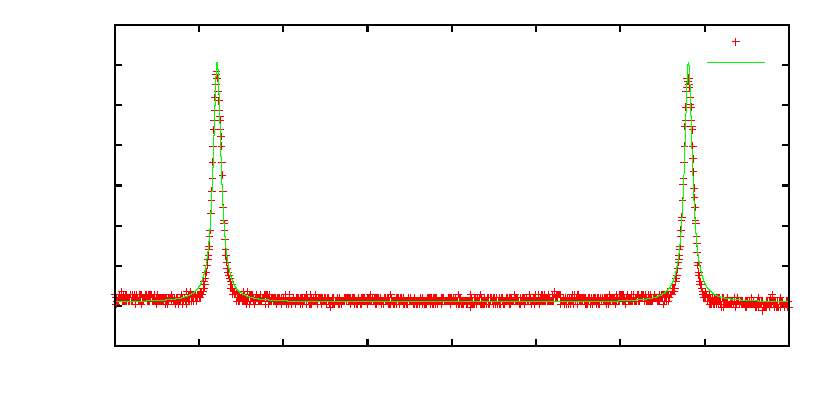
\includegraphics{finesse_messung_a}}%
    \gplfronttext
  \end{picture}%
\endgroup
